%% LaTeX-Beamer template for KIT design
%% by Erik Burger, Christian Hammer
%% title picture by Klaus Krogmann
%%
%% version 2.1
%%
%% mostly compatible to KIT corporate design v2.0
%% http://intranet.kit.edu/gestaltungsrichtlinien.php
%%
%% Problems, bugs and comments to
%% burger@kit.edu

\documentclass[18pt]{beamer}

%% SLIDE FORMAT

% use 'beamerthemekit' for standard 4:3 ratio
% for widescreen slides (16:9), use 'beamerthemekitwide'

\usepackage{templates/beamerthemekit}
% \usepackage{templates/beamerthemekitwide}

%% TITLE PICTURE

% if a custom picture is to be used on the title page, copy it into the 'logos'
% directory, in the line below, replace 'mypicture' with the
% filename (without extension) and uncomment the following line
% (picture proportions: 63 : 20 for standard, 169 : 40 for wide
% *.eps format if you use latex+dvips+ps2pdf,
% *.jpg/*.png/*.pdf if you use pdflatex)

%\titleimage{mypicture}

%% TITLE LOGO

% for a custom logo on the front page, copy your file into the 'logos'
% directory, insert the filename in the line below and uncomment it

% \titlelogo{mylogo}

% (*.eps format if you use latex+dvips+ps2pdf,
% *.jpg/*.png/*.pdf if you use pdflatex)

%% TikZ INTEGRATION

% use these packages for PCM symbols and UML classes
% \usepackage{templates/tikzkit}
% \usepackage{templates/tikzuml}

% the presentation starts here

\title[Short title]{Shellshock\\ With all details}
\subtitle{Proseminar - Aktuelle IT-Sicherheitsvorf\"alle und L\"osungsans\"atze}
\author{Martin Weiss, Kay Schmitteckert}

\institute{Forschungsgruppe Dezentrale Systeme und Netzdienste - TM \& SCC}

% Bibliography
\usepackage[utf8]{inputenc}
\usepackage[citestyle=authoryear,bibstyle=numeric,hyperref,backend=biber]{biblatex}
\addbibresource{templates/example.bib}
\bibhang1em
\setcounter{tocdepth}{1}

\begin{document}

% change the following line to "ngerman" for German style date and logos
\selectlanguage{ngerman}

%title page
\begin{frame}
\titlepage
\end{frame}

%table of contents
\begin{frame}{Agenda}
\tableofcontents
\end{frame}

\section{Shellshock}
\begin{frame}{Shellshock}
\begin{block}{Was ist Shellshock?}
  \begin{itemize}[<+->]
    \item Bash Sicherheitslücke
    \item Entdeckung September 2014
    \item Existiert seit 1989
    \item CVE-Nummern CVE-2014-6271, -7169, -7168, -7187, -6277, -6278
    \item 3 Patches bis zur Behebung
  \end{itemize}
\end{block}
\end{frame}

\begin{frame}{Shellshock}
\begin{block}{Ausmaß des Exploits}
\begin{itemize}[<+->]
\item Bash Standard-Shell bei vielen unixoiden Systemen
\item Großteil der Webserver laufen unter unixoiden Systemen
\item Weltweit waren hunterte Millionen Computer betroffen
\begin{itemize}
  \item Unter anderem Server von Yahoo, Winzip und Lycos
\end{itemize}
\item Forscher halten die Sicherheitslücke für gravierender als Heartbleed
\end{itemize}
\end{block}
\end{frame}

\begin{frame}{Ungepatchte Bash}
\begin{figure}
  \centering
    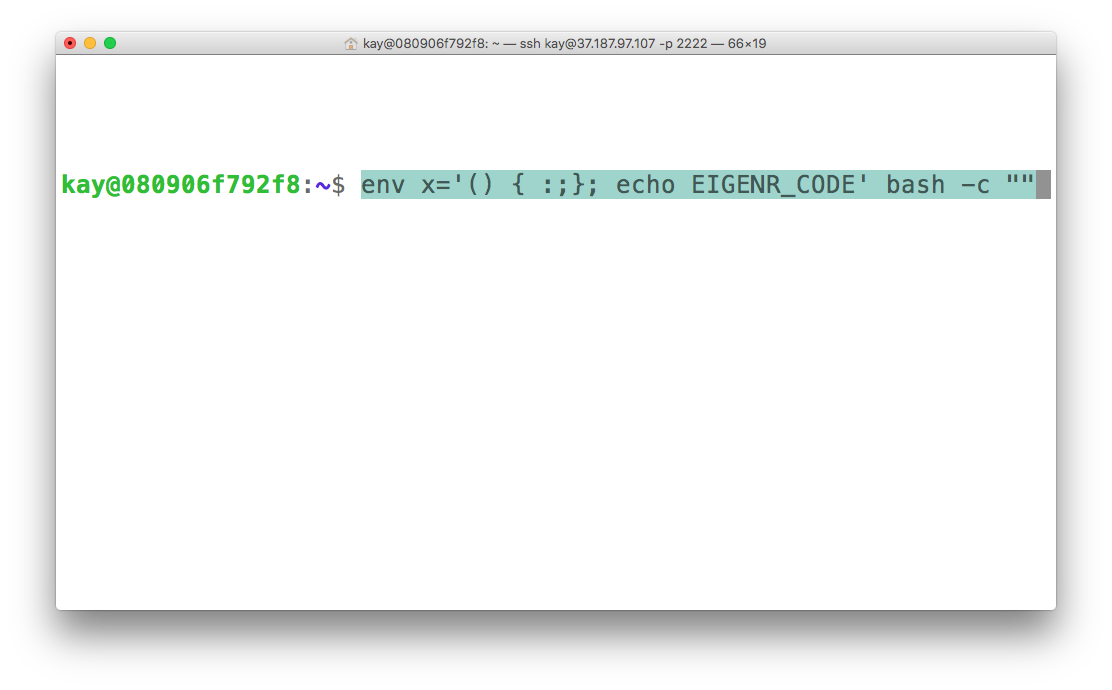
\includegraphics[width=1\textwidth]{assets/example1}
\end{figure}
\end{frame}

\begin{frame}{Ungepatchte Bash}
\begin{figure}
  \centering
    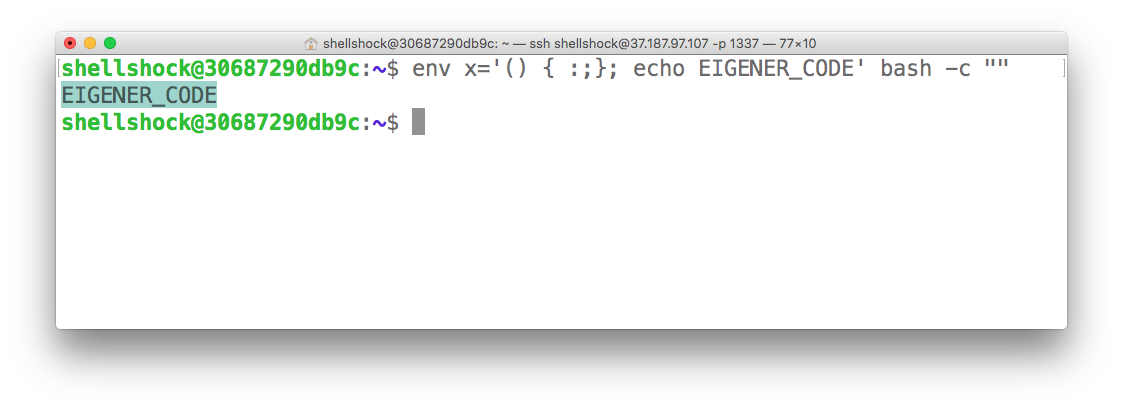
\includegraphics[width=1\textwidth]{assets/example2}
\end{figure}
\end{frame}

\section{Hätte man Shellshock vorbeugen können?}
\begin{frame}{Vorbeugung von Shellshock möglich?}
\begin{center}
\begin{Huge}
Ja!
\end{Huge}
\end{center}
\end{frame}

\section{Hätte man Shellshock vorbeugen können?}
\begin{frame}{Vorbeugung von Shellshock möglich?}
\begin{block}{Möglichkeiten}
\begin{itemize}[<+->]
\item Präventive Verteidigungsmaßnahmen
\pause
\item Maßnahmen gegen SQL-Injections
\item \dots
\end{itemize}
\end{block}
\end{frame}

\section{Präventive Verteidigungsmaßnahmen}
\begin{frame}{Präventive Verteidigungsmaßnahmen}
\begin{exampleblock}{Möglichkeiten}
\begin{itemize}
\item Präventive Verteidigungsmaßnahmen
\pause
\item Maßnahmen gegen SQL-Injections
\item \dots
\end{itemize}
\end{exampleblock}
\end{frame}


\section{Maßnahmen gegen SQL-Injections}

\begin{frame}{SQL-Injections}
\begin{block}{Generelles}
\begin{itemize}
	\item Stellen seit Einführung von Datenbanken ein Sicherheitsrisiko dar
	\item Machen ca. 69\% aller Angriffe aus \footnotemark
	\item Benutzereingaben werden in der SQL-Abfrage missinterpretiert
\end{itemize}
\end{block}
\setbeamerfont{footnote}{size=\tiny}
\footnotetext{Stand: Q2 2012; Quelle: http://www.zdnet.com/article/sql-injection-attacks-up-69/}
\setbeamerfont{footnote}{size=\footnotesize}
\end{frame}

\begin{frame}{Klassische Angriffe}
\begin{block}{Numerische SQL-Abfrage}
	SELECT * FROM Users WHERE ID = \textcolor{red}{\textbf{1 OR 1=1}}
\end{block}
\begin{block}{SQL-Abfrage mit String-Wert}
	SELECT * FROM Users WHERE name = '{}\textcolor{red}{\textbf{nickname'{} OR 1=1- -}}'{}
\end{block}
\end{frame}


\begin{frame}{Maßnahmen gegen SQL-Injections}
\begin{block}{Lösungsansätze}
\begin{itemize}
\item Blacklisting 
\item Whitelisting
\item Escaping
\item Prepared Statements \& Bind Variablen
\end{itemize}
\end{block}
\end{frame}

\begin{frame}{Blacklisting}
\begin{block}{Vorgehen}
\begin{itemize}
\item Benutzereingaben werden gefiltert
	\begin{itemize}
	\item Metazeichen von der Eingabe entfernen (z.B.: ", ;, ', -, \%)
	\item Getrimmter Substring wird im SQL-Query verwendet
	\end{itemize}
\end{itemize}
\end{block}
\begin{block}{Beispiel}	
	remove\_metachar("{}\textcolor{red}{\textbf{nickname'{} OR 1=1- -}}{}") $\Rightarrow$ "{}\textcolor{red}{\textbf{nicknameOR1=1}}{}" \\
	$\Rightarrow$ SELECT * FROM Users WHERE name = '{}\textcolor{red}{\textbf{nicknameOR1=1}}'{}

\end{block}
\end{frame}

\begin{frame}{Blacklisting}
\begin{block}{Vorgehen}
\begin{itemize}
\item Benutzereingaben werden gefiltert
	\begin{itemize}
	\item Metazeichen von der Eingabe entfernen (z.B.: ", ;, ', -, \%)
	\item Getrimmter Substring wird im SQL-Query verwendet
	\end{itemize}
\end{itemize}
\end{block}
\begin{block}{Problematik \& Sicherheit}	
\begin{itemize}
\item Vergessen von einem einzigen Metacharakter kann kompletten Lösungsansatz zerstören
\end{itemize}
\end{block}
\end{frame}


\begin{frame}{Whitelisting}
\begin{block}{Vorgehen}
\begin{itemize}
	\item Nur gültige Zeichen zulassen
	\item Validierung \& Überprüfung mittels regulärem Ausdruck
\end{itemize}	
\end{block}
\begin{block}{Beispiel}	
	Whitelist: [0,9]* \\
	check\_whitelist("{}\textcolor{red}{\textbf{1 OR 1=1}}{}") $\mapsto$ "{}\textcolor{red}{\textbf{ungültige Eingabe}}{}" \\
	trim\_whitelist("{}\textcolor{red}{\textbf{1 OR 1=1}}{}") $\mapsto$ "{}\textcolor{red}{\textbf{ungültige Eingabe}}{}" \\
	$\Rightarrow$ SELECT * FROM Users WHERE ID = \textcolor{red}{\textbf{1}}
\end{block}
\end{frame}

\begin{frame}{Whitelisting}
\begin{block}{Vorgehen}
\begin{itemize}
	\item Nur gültige Zeichen zulassen
	\item Validierung \& Überprüfung mittels regulärem Ausdruck
\end{itemize}	
\end{block}
\begin{block}{Problematik \& Sicherheit}	
\begin{itemize}
\item Herr O'Neil kann sich nicht mehr mit seinem Namen registrieren
\end{itemize}
\end{block}
\end{frame}


\begin{frame}{Escaping}
\begin{block}{Vorgehen}
\begin{itemize}
\item Benutzereingabe wird so umgeformt, dass die Datenbank sie richtig interpretieren kann
\item Funktioniert nur bei String-Eingaben
\end{itemize}
\end{block}
\begin{block}{Beispiel}
	escape("{}\textcolor{red}{\textbf{O'Neil}}"{}) $\mapsto$ "{}\textcolor{red}{\textbf{O"{}Neil}}"{} \\
	$\Rightarrow$ Datenbank interpretiert "{} als einfaches ' und nicht mehr als Beginn bzw. Ende eines Strings
\end{block}
\end{frame}

\begin{frame}{Escaping}
\begin{block}{Vorgehen}
\begin{itemize}
\item Benutzereingabe wird so umgeformt, dass die Datenbank sie richtig interpretieren kann
\item Funktioniert nur bei String-Eingaben
\end{itemize}
\end{block}
\begin{block}{Problematik \& Sicherheit}
\begin{itemize}
\item escape()-Funktion muss konsistent und überall (bei INSERT, UPDATE, DELETE, etc.) angewendet werden
\item Ermöglicht sonst Second Order SQL-Injections
\end{itemize}
\end{block}
\end{frame}

\begin{frame}{Prepared Statements \& Bind Variablen}
\begin{block}{Vorgehen}
\begin{itemize}
\item Nutzen von Platzhaltern (z.B.: ?, :name, etc.) anstatt Eingaben direkt in der Datenbank-Abfrage zu verwenden
\item Query wird zuerst vorbereitet und danach erst die Parameter eingesetzt
\end{itemize}
\end{block}
\begin{block}{Beispiel}
prep\_stat = "{}SELECT * FROM Users WHERE ID = \textcolor{red}{\textbf{?}} AND name = \textcolor{red}{\textbf{?}}"{}; \\
prep\_stat.setPara(1, "{}\textcolor{red}{\textbf{1 OR 1=1}}{}"); \\
prep\_stat.setPara(2, "{}\textcolor{red}{\textbf{nickname'{} OR 1=1- -}}{}"); \\
prep\_stat.exec\_query;
\end{block}
\end{frame}

\begin{frame}{Prepared Statements \& Bind Variablen}
\begin{block}{Vorgehen}
\begin{itemize}
\item Nutzen von Platzhaltern (z.B.: ?, :name, etc.) anstatt Eingaben direkt in der Datenbank-Abfrage zu verwenden
\item Query wird zuerst vorbereitet und danach erst die Parameter eingesetzt
\end{itemize}
\end{block}
\begin{block}{Problematik \& Sicherheit}
\begin{itemize}
	\item Durch Platzhalter kann der Angreifer die SQL-Abfrage nicht verändern
	\item Die SQL-Abfrage kann nicht missinterpretiert werden
	\item Fast unmöglich die Abfrage zu manipulieren
	\item Bester Ansatz, um SQL-Injections zu vermeiden
\end{itemize}
\end{block}
\end{frame}



\section{Fazit und Resümee}
\begin{frame}{Fazit und Resümee}
\begin{block}{Möglichkeiten}
\begin{itemize}[<+->]
\item Präventive Verteidigungsmaßnahmen
\pause
\item Maßnahmen gegen SQL-Injections
\item \dots
\end{itemize}
\end{block}
\end{frame}

\end{document}
